\catcode`\_=13 
\def_{\textunderscore}
\catcode`_=8

\chapter{Genereller Ablauf des Projekts}\addtocontents{lof}{\vspace{3mm}}\addtocontents{lol}{\vspace{3mm}}
Der Kurs wird in Gruppen unterteilt, die Gruppenleiter sind markiert:\\
\begin{tabular}[h]{|c|c|c|c|}
	\hline
	\textbf{Organisation} & \textbf{Coding} & \textbf{Design} & \textbf{Dokumentation} \\
	\hline
	Dengler, Denis & Bröcker, Alexander & Ehmer, Anna-Lena & Schader, David \\
	Lange, Johannes & Göl, Onur & Fuchs, Julian & \textbf{Scheffler, Martina} \\
	Pankewitsch, Franziska & Henkel, David & Kürschner, Maximilian &\\
	Reichert, Anne & Kreutz, Julian & Michel, Elisa &\\
	& Rhmmo, Ahmad & \textbf{Rosenbach, Lukas} &\\
	& \textbf{Risch, David} & Seus, Dominik &\\
	& Wallat, Sebastian & von der Lehr, Fabrice &\\
	& Weinmann, Felix & Wolf, Dennis &\\
	\hline
\end{tabular}
\\\\Eine weitere Gruppe \textbf{Test} ist im späteren Verlauf des Projekts geplant bleibt aber erstmal leer.
\\\\
Zu Beginn wird festgelegt, was das Thema des Projekts ist, die Abstimmung darüber leitet das Organisationsteam.

\chapter{Thema des Projekts}
Das Ziel des Projekts ist die Entwicklung einer Anwendung zum Verwalten des Alltags in einer WG.\\
Weiterer Bestandteil der Anwendung ist eine "Tischkicker-App".\\\\
Zur weiteren Organisation des Projekts wurden User Stories und Tasks formuliert und geschätzt. Diese sind \href{https://studentdhbwmannheimde-my.sharepoint.com/personal/s181108_student_dhbw-mannheim_de/_layouts/15/onedrive.aspx?originalPath=aHR0cHM6Ly9zdHVkZW50ZGhid21hbm5oZWltZGUtbXkuc2hhcmVwb2ludC5jb20vOmY6L2cvcGVyc29uYWwvczE4MTEwOF9zdHVkZW50X2RoYnctbWFubmhlaW1fZGUvRXNFbnRKWC11VkpHa1N5MFZySWVxaHdCV2pQcl9MMzg3c0h3UUZvODJhZFVJZz9ydGltZT1xYkhMZm9yYzEwZw&viewid=7833eb22%2Db78c%2D4ca2%2D847f%2Dce9bd5826118&id=%2Fpersonal%2Fs181108%5Fstudent%5Fdhbw%2Dmannheim%5Fde%2FDocuments%2FVorlesungen%2F3%2E%20Semester%2FSoftware%2DEngineering%2FProjekt%2FArchiv}{hier}
zu finden.

\chapter{Arbeit am Projekt}
Hier werden jede Woche die getroffenen Beschlüsse der Gruppenarbeit festgehalten.
\section{Design}
\subsection{Beschlüsse aus dem 3. Semester}
Als Farben für die Oberfläche wurden schwarz und türkis gewählt.
	\begin{figure}[h!]
		\centering
		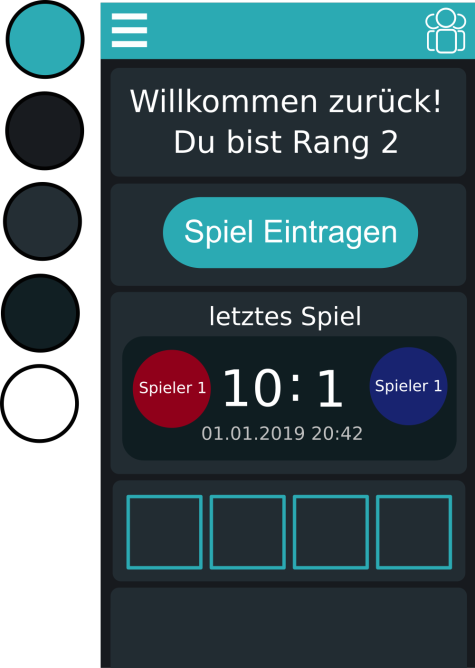
\includegraphics[width=0.5\linewidth]{text/Farben_des_Designs}
		\caption{Farbdesign}
		\label{farbdesign}
	\end{figure}
\subsection{Di, 07.04.2020}
Die Darstellung der Datenbank übernehmen das Design- und das Organisationsteam gemeinsam.\\
Des weiteren, soll jedes Mitglied des Designteams - ausgehend vom Farbdesign aus dem dritten Semester (Abbildung \ref{farbdesign}) - eine Startseite entwerfen, über diese wird in der nächsten Vorlesung entschieden.
Von dieser ausgehend werden dann die weiteren Ansichten entworfen.\\
Zum Design von Entwürfen soll \href{https://www.figma.com/}{figma.com} verwendet werden.
\subsection{Di, 14.04.2020}
	\begin{figure}[h!]
		\centering
		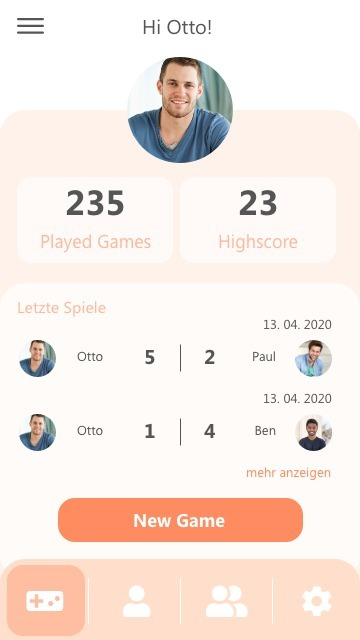
\includegraphics[width=0.4\linewidth]{text/Startseite}
		\caption{Startseite}
		\label{startseite}
	\end{figure}
Das abgebildete Schema für die Startseite (Abbildung \ref{startseite}) wurde mehrheitlich beschlossen. Da dieses aber noch nicht dem eigentlichen Farbdesign entspricht, wird dieses bis zur nächsten Woche noch einmal überarbeitet.\\
Neben der Festlegung auf dieses Schema für die Startseite wurden auf die Gruppenmitglieder der Design-Gruppe die Aufgaben verteilt, im Laufe der Woche bestimmte Ansichten zu entwerfen. Dazu gehören folgende Ansichten:\\
\begin{itemize}
	\item Erstellen einer Gruppe
	\item Anmelden
	\item Registrieren
	\item Erstellen eines Turniers
	\item Eintragen der Ergebnisse
	\item Statistiken
	\item Verwaltung des Profils
	\item Laufendes Turnier
\end{itemize}
\begin{figure}[h!]
		\centering
		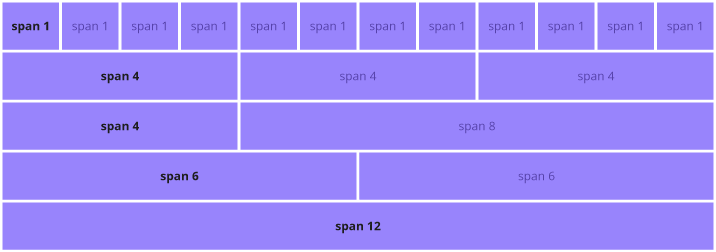
\includegraphics[width=0.9\linewidth]{text/design_gridsystem}
		\caption{Gridsystem}
		\label{gridsystem}
	\end{figure}
Zusätzlich wurde für das Design ein Gridsystem (Abbildung \ref{gridsystem}) beschlossen. Demnach können in den Ansichten einzelne Zeilen in bis zu 12 Teile aufgeteilt werden, dies erleichtert eine einheitliche Gestaltung.
\subsection{Di, 21.04.2020}
Da die erstellten Designentwürfe noch keinem einheitlichen Schema entsprechen, wurden Angaben für die Überarbeitung der Designentwürfe der einzelnen Ansichten besprochen.
Zunächst wurde dazu eine svg-Datei als Template zur Verfügung gestellt am Beispiel der Ansicht des Testtuniers (Abbildung \ref{template}).\\
\begin{figure}[h!]
	\centering
	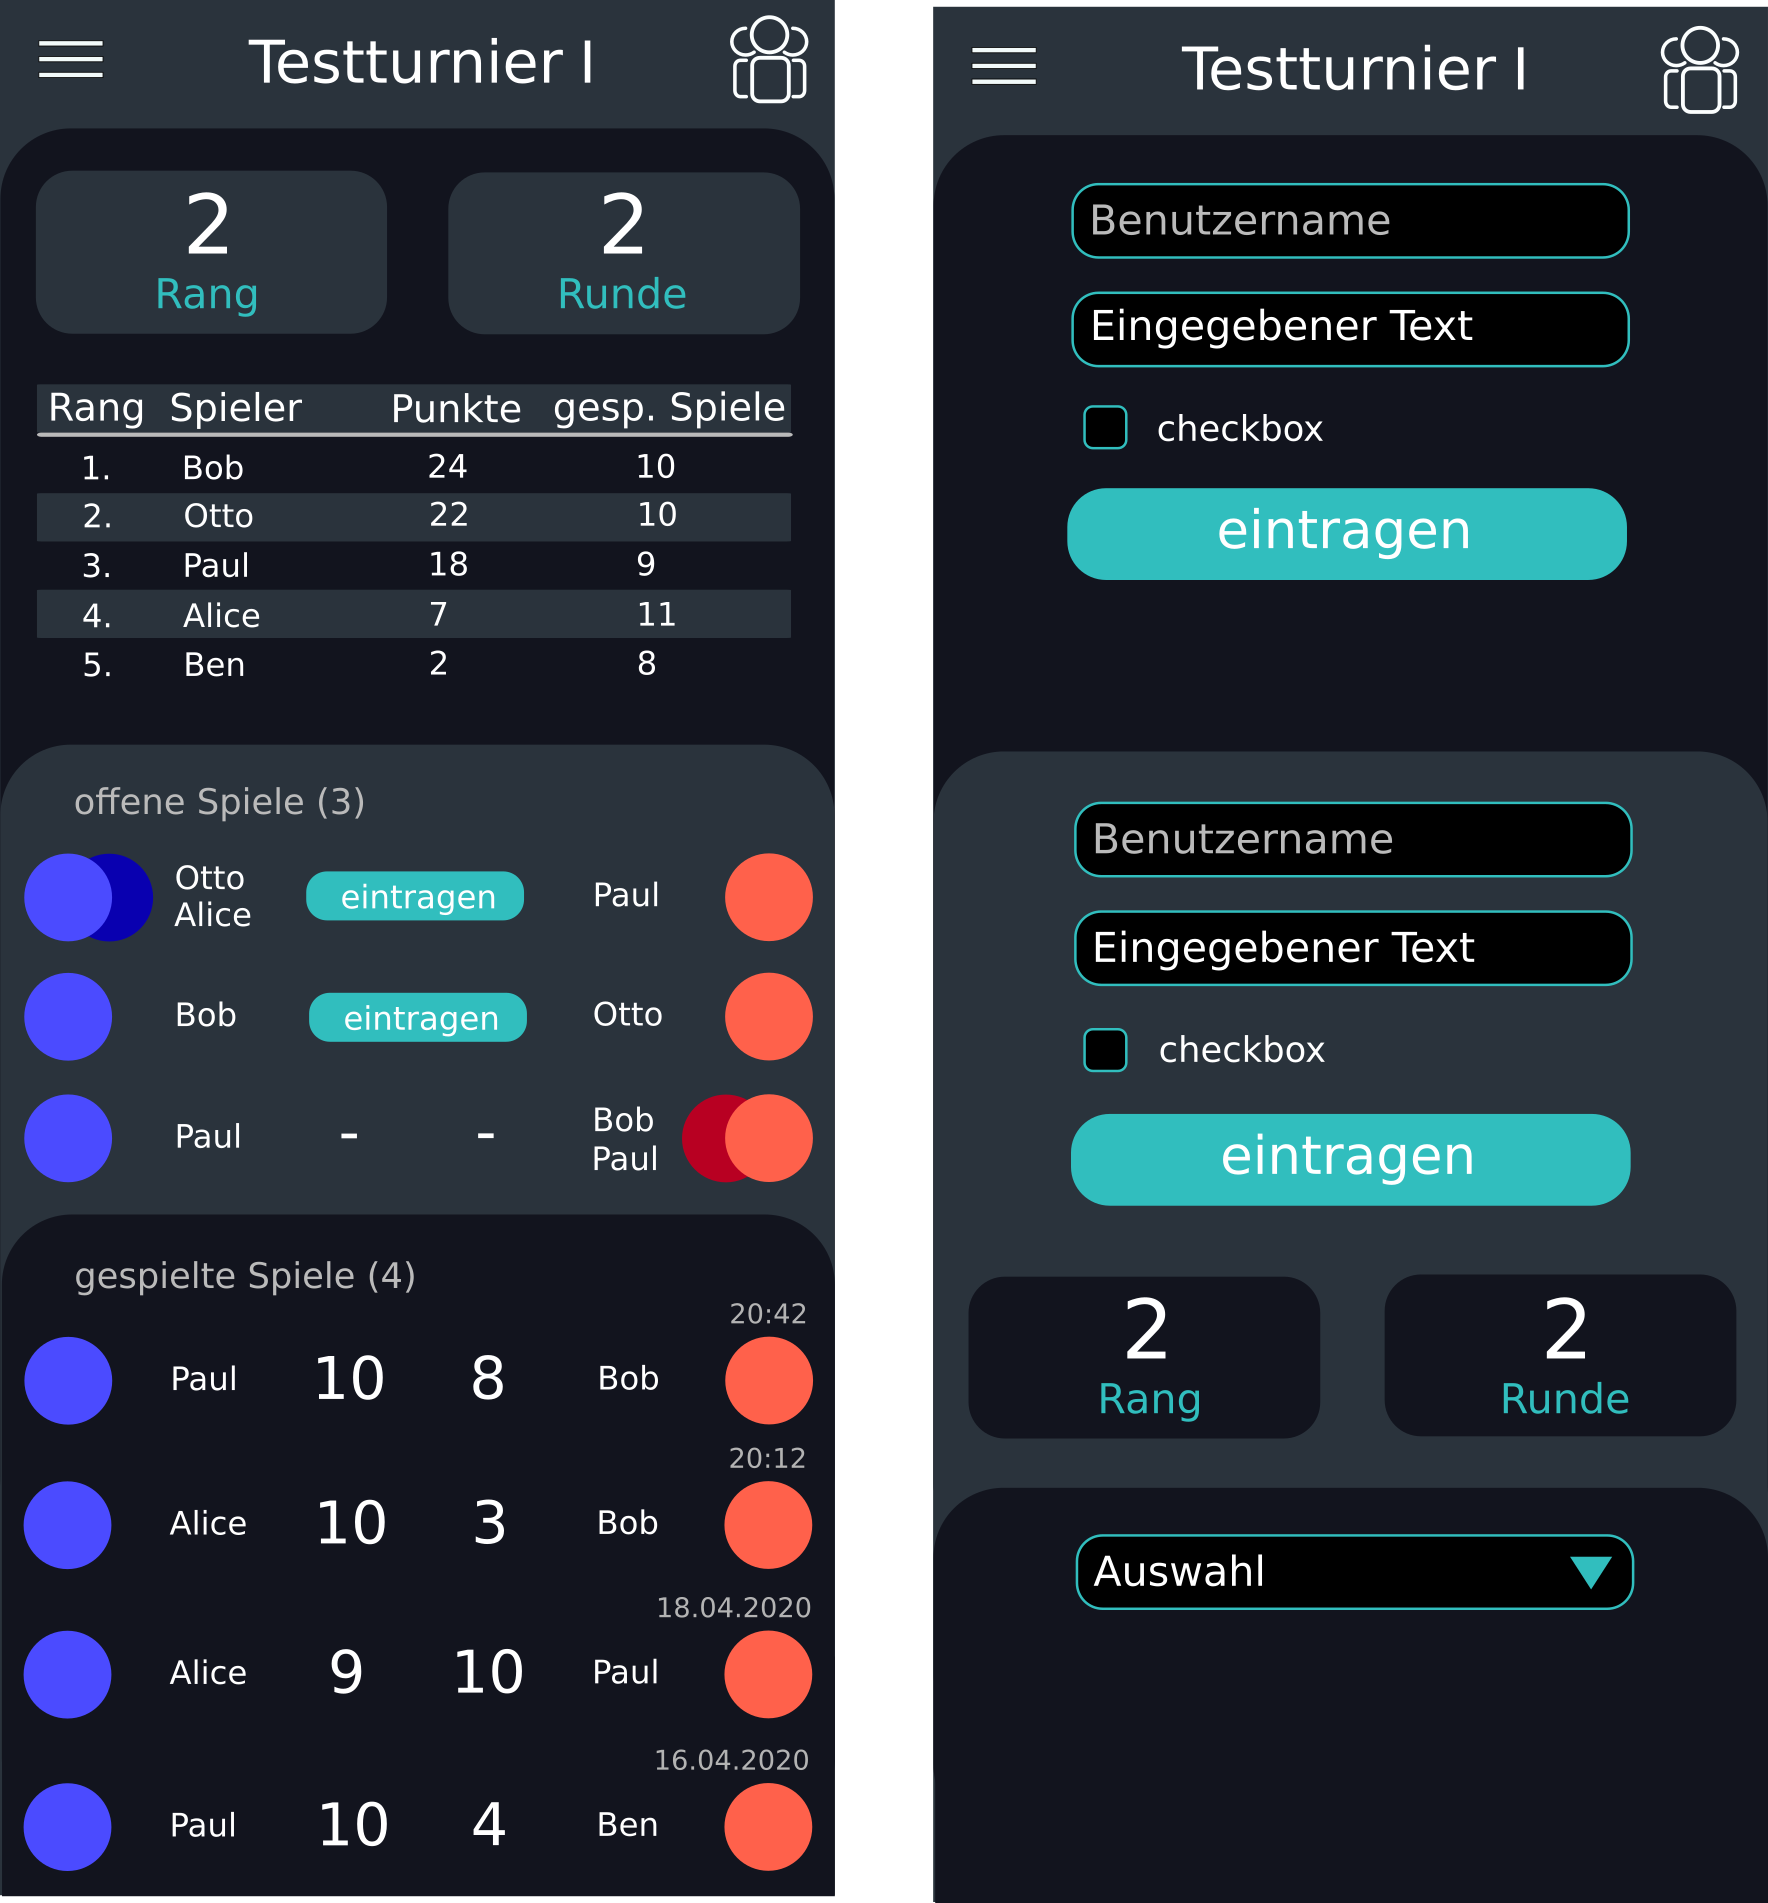
\includegraphics[width=0.6\linewidth]{text/Template}
	\caption{Template}
	\label{template}
\end{figure}
Zusätzlich wurden Farbwerte für die Designs in RGBA-Werten und die verwendete Schriftart angegeben:
\begin{itemize}
	\item Hintergrundfarben:
	\begin{itemize}
		\item Hellgrau: 2a333cff
		\item Dunkelgrau: 12141eff
		\item Türkis: 31bebeff
	\end{itemize}
	\item Schriftfarben:
	\begin{itemize}
		\item Weiß: ffffffff
		\item Türkis: 31bebeff
		\item Grau: bababaff
	\end{itemize}
	\item Eingabefeld:
	\begin{itemize}
		\item Schwarz: 000000ff
		\item Türkis: 31bebeff
	\end{itemize}
	\item Schriftart: sans-serif
\end{itemize}
Da auch noch einige Ansichten fehlten, werden von einzelnen Team-Mitgliedern Designs für folgende Ansichten entworfen:
\begin{itemize}
	\item Gruppe verwalten
	\item Letzte Spiele
	\item Beendetes Turnier
	\item Achievements
	\item FAQ
\end{itemize}
\subsection{Di, 28.04.20}
Der Entwurf der Datenbank (Abbildung \ref{DB}) wurde vorgestellt und besprochen.
\begin{figure}[h!]
	\centering
	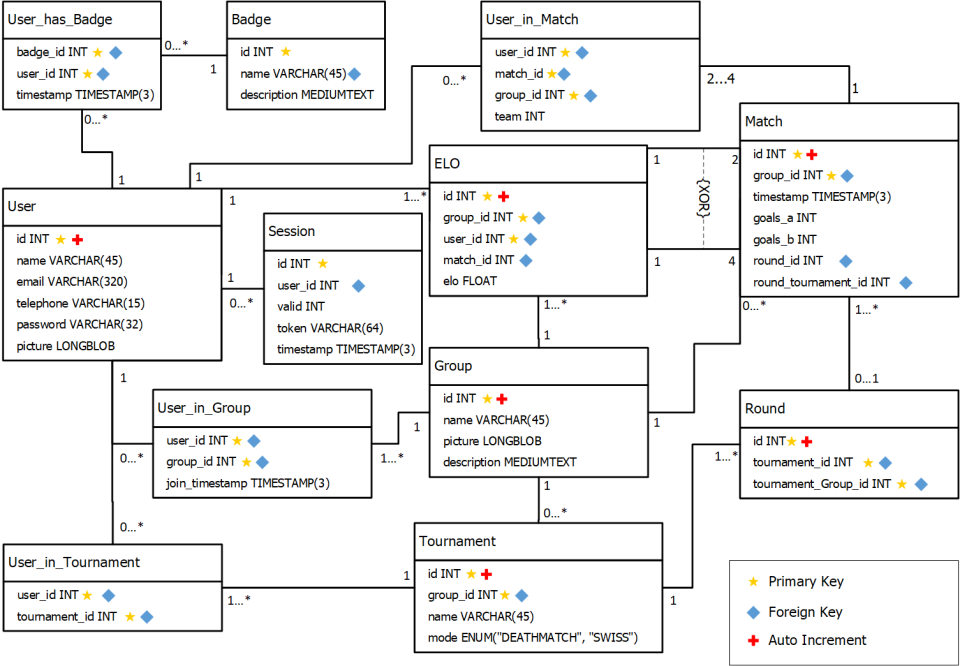
\includegraphics[width=\linewidth]{text/Datenbankmodell}
	\caption{Datenbankentwurf}
	\label{DB}	
\end{figure}
\\Die finalen Designansichten sind nun \href{https://studentdhbwmannheimde-my.sharepoint.com/:f:/g/personal/s181108_student_dhbw-mannheim_de/Ek6DMqY0oCdFnB_9TndCsqAB3wNP20j2XAipOnYleT43Vw?e=0DY5WZ}{hier} einzusehen.
\\Für die Implementierung werden diese Designansichten in ein css-Format gebracht, damit das Coding-Team die Ansichten einbinden kann. Zusätzlich werden noch Designentwürfe mit dem dazugehörigen css-Format für folgende Ansichten entworfen:
\begin{itemize}
	\item Burgermenü
	\item Gruppenauswahl
	\item Spielerauswahl
	\item Bildkreis
	\item Spielzeile
	\item Alte Turniere
	\item Impressum
	\item Ansichten beim ersten Öffnen der App (Anmelden, Registrieren, Logo)
\end{itemize}



\newpage
\section{Coding}
\subsection{Di, 07.04.2020}
Als IDE soll Webstorm verwendet werden.\\
Ein \href{https://github.com/DavidRisch/kicker}{Github-Repository} wurde angelegt, dort sind im Wiki auch die Tasks, die im dritten Semester beschlossen wurden, zu finden.
\subsection{Di, 14.04.2020}
Die Struktur des Github-Repositorys ist wie folgt:
	\begin{itemize}
		\item \textit{api}: js files for backend post requests, returns json
		\item \textit{css}: all css files
		\item \textit{html}: all html files, mostly for use in \textit{pages/}
		\item \textit{js}: js files for use in the client browser
		\item \textit{page}: js files generating html on get requests
		\item \textit{src}: js files for importing in other javascript files
		
	\end{itemize}
\subsection{Di, 21.04.2020}
Erste Tasks, für die die Datenbank nicht nötig ist, wurden bereits bearbeitet.
Nach endgültiger Beschprechung der Datenbankstruktur, kann ab nächster Woche mit dem Hauptaufwand der Programmierung begonnen werden.
\subsection{Di, 28.04.2020}
Ab hier sind alle nötigen Vorraussetzungen für die Programmierung vorhanden und die Tasks werden abgearbeitet.
\newpage
\section{Organisation}
\subsection{Impressum}
Das Impressum wurde wie folgt festgelegt:\\\\
\textbf{Impressum}\\
Diese Website wurde im Rahmen der Vorlesung Software Engineering der DHBW Mannheim entwickelt.\\\\
Angaben gemäß §5 TMG\\\\
DHBW Mannheim\\
(Duale Hochschule Baden-Württemberg Mannheim)\\
Coblitzallee 1-9\\
68163 Mannheim\\\\
\textbf{Projektbetreuung}\\
Herr Schultheis\\\\
\textbf{Kontakt}\\
Telefon: +49 621 4105-0\\
E-Mail: info@dhbw-mannheim.de

\chapter{Use Cases und Aktivitätsdiagramme}
\section{Registrierung und Anmeldung}
\begin{figure}[h!]
	\centering
	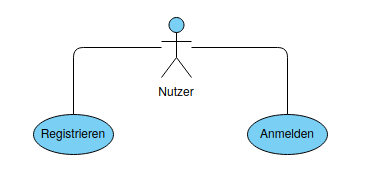
\includegraphics{text/registrierung_anmeldung.png}
	\caption{Use Case: Registrierung und Anmeldung}
	\label{uc_reg_anm}
\end{figure}
\textbf{Registrieren}
\begin{itemize}
	\item \textbf{Use Case:} Registrieren
	\item \textbf{Ziel:} Registriert
	\item \textbf{Kategorie:} Primär
	\item \textbf{Vorbedingung:} Nutzer hat bisher kein Konto
	\item \textbf{Nachbedingung Erfolg:} Konto angelegt
	\item \textbf{Nachbedingung Fehlschlag:} Konto nicht anlegbar
	\item \textbf{Akteure:} Nutzer
	\item \textbf{Auslösendes Ereignis:} Nutzer beendet Registrierungsprozess
	\item \textbf{Beschreibung:} \begin{enumerate}
		\item Eingegebenen Namen auf erlaubte Eingabewerte überprüfen
		\item Überprüfung, ob eingegebener Name bisher unbekannt ist
		\item E-Mail-Adresse auf erlaubte Eingabewerte überprüfen
		\item Überprüfung, ob eingegebene E-Mail-Adresse bisher unbekannt ist
		\item Eingegebenes Passwort auf erlaubte Eingabewerte überprüfen
		\item Telefonnummer auf reine Verwendung von Zahlen überprüfen
		\item Überprüfen, ob Datenschutzbedingungen akzeptiert wurden
		\item Eintragen der angegebenen Werte in die Datenbank
	\end{enumerate}
	\item \textbf{Erweiterungen:} /
	\item \textbf{Alternativen:} /
\end{itemize}


\textbf{Anmelden}
\begin{itemize}
	\item \textbf{Use Case:} Anmelden
	\item \textbf{Ziel:} Angemeldet
	\item \textbf{Kategorie:} Primär
	\item \textbf{Vorbedingung:} Nutzer hat bereits ein Konto
	\item \textbf{Nachbedingung Erfolg:} Nutzer ist am Server authentifiziert
	\item \textbf{Nachbedingung Fehlschlag:} Nutzer konnte nicht am Server authentifiziert werden
	\item \textbf{Akteure:} Nutzer
	\item \textbf{Auslösendes Ereignis:} Nutzer beendet Anmeldeprozess
	\item \textbf{Beschreibung:} \begin{enumerate}
		\item Nutzer an eingegebenem Namen bestimmen
		\item Nutzer mit eingegebenem Passwort identifizieren
		\item Nutzer auf Startseite weiterleiten
	\end{enumerate}
	\item \textbf{Erweiterungen:} /
	\item \textbf{Alternativen:} 1a. Nutzer an eingegebener E-Mail-Adresse bestimmen
\end{itemize}
\clearpage
\begin{figure}[h!]
	\centering
	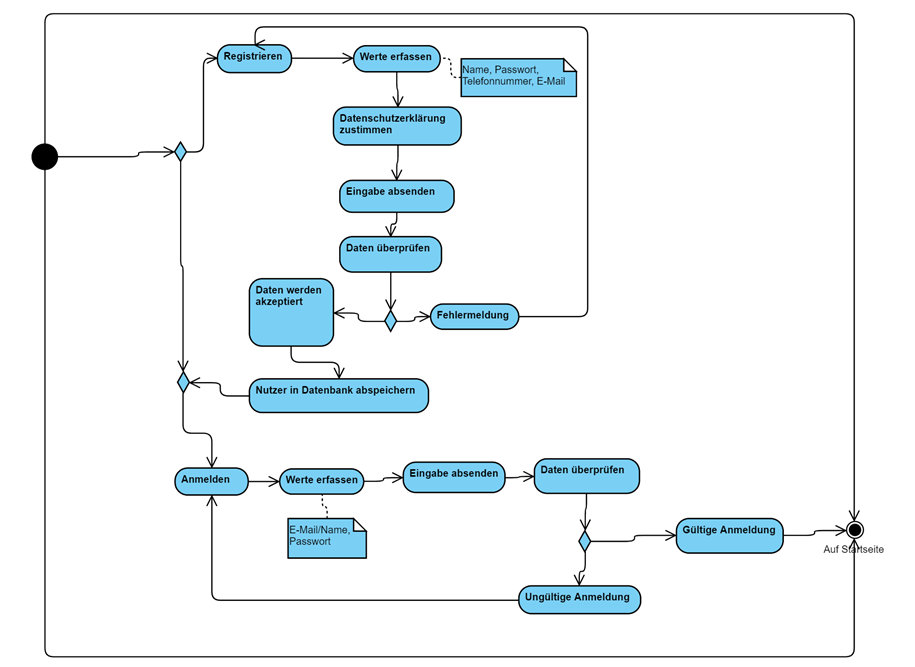
\includegraphics[width=\linewidth]{text/aktiv_reg_anm.png}
	\caption{Aktivitätsdiagramm: Registrierung und Anmeldung}
	\label{ak_reg_anm}
\end{figure}


\section{Turniererstellung}
\begin{figure}[h!]
	\centering
	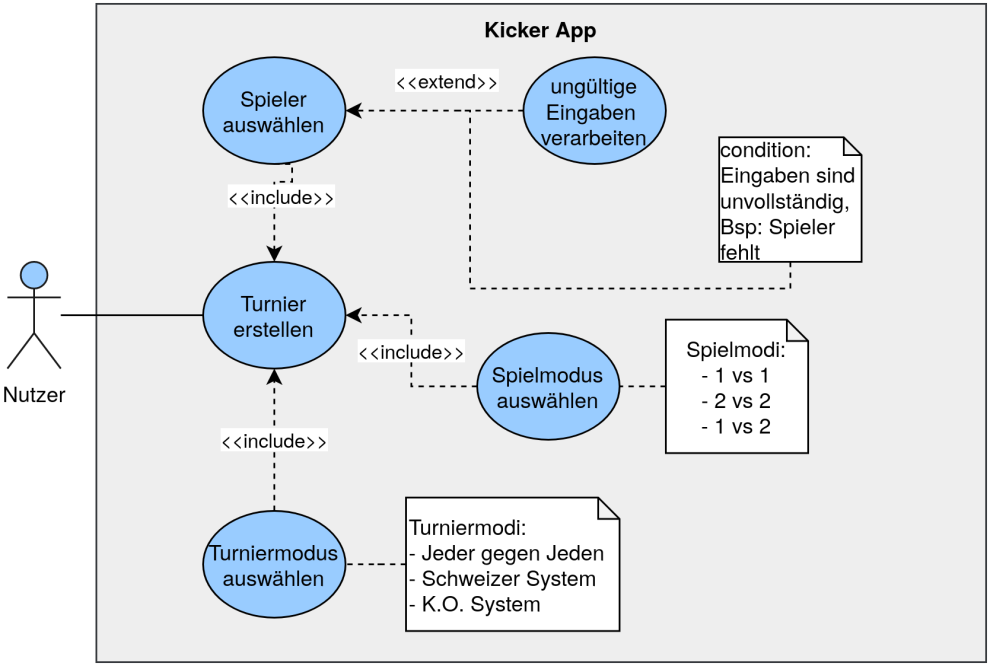
\includegraphics[width=\linewidth]{text/uc_turnier.png}
	\caption{Use Case: Turniererstellung}
	\label{uc_turnier}
\end{figure}
\begin{itemize}
	\item \textbf{Use Case:} Turnier erstellen
	\item \textbf{Ziel:} Erstellen eines Turniers und Wechsel zur Turnieransicht
	\item \textbf{Kategorie:} Primär
	\item \textbf{Vorbedingung:} Nutzer hat ein Konto und ist angemeldet
	\item \textbf{Nachbedingung Erfolg:} Turnieransicht wird geöffnet und die angegebenen Teilnehmer werden benachrichtigt
	\item \textbf{Nachbedingung Fehlschlag:} Turnier wird nicht erstellt, es wird eine erneute Eingabe der Daten gefordert
	\item \textbf{Akteure:} Nutzer
	\item \textbf{Auslösendes Ereignis:} Nutzer klickt auf Link "Turnier erstellen" in der Seitenleiste oder auf der Startseite
	\item \textbf{Beschreibung:} \begin{enumerate}
		\item Eingabe eines Namens für das Turnier
		\item Auswahl des Spielmodus
		\item Auswahl des Turniermodus
		\item Auswahl der Mitspieler
		\item Absenden der Eingaben führt zur Erstellung des Turniers
	\end{enumerate}
	\item \textbf{Erweiterungen:} /
	\item \textbf{Alternativen:} Die Ausführungsschritte 2.-4. können in beliebiger Reihenfolge ausgeführt werden
\end{itemize}


\section{Spielerstellung}
\begin{figure}[h!]
	\centering
	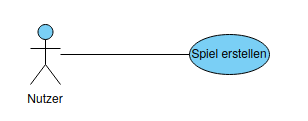
\includegraphics{text/uc_spiel.png}
	\caption{Use Case: Spielerstellung}
	\label{uc_spiel}
\end{figure}
\begin{figure}[h!]
	\centering
	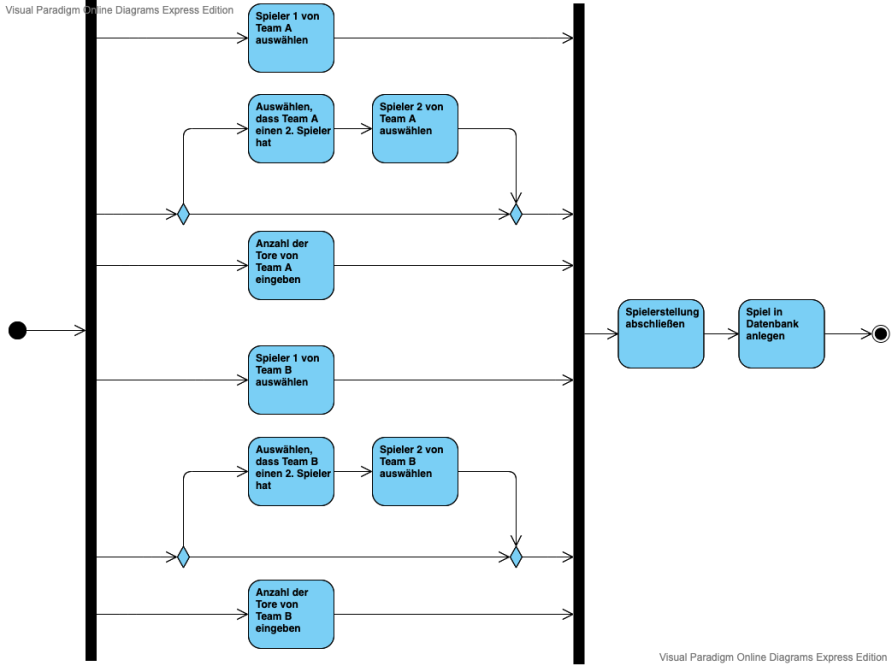
\includegraphics[width=\linewidth]{text/aktiv_spiel.png}
	\caption{Aktivitätsdiagramm: Spielerstellung}
	\label{aktiv_spiel}
\end{figure}


\section{Gruppenerstellung}
\begin{figure}[h!]
	\centering
	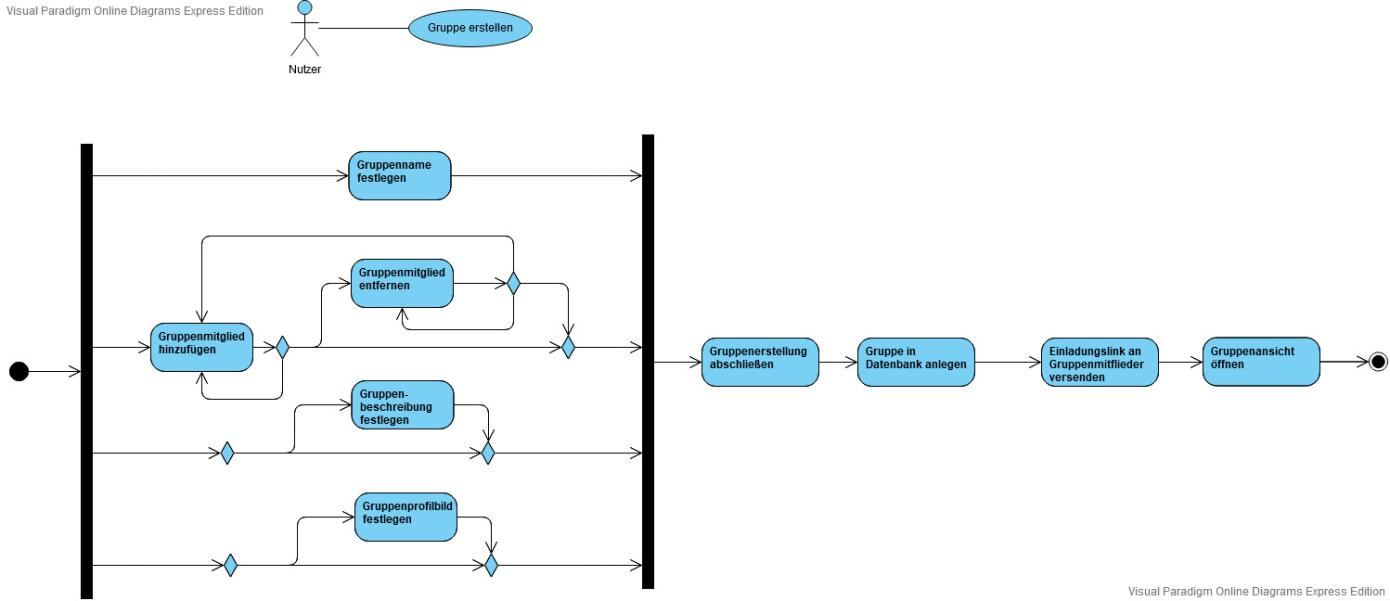
\includegraphics[width=\linewidth]{text/uc_ak_gruppenerstellung.jpg}
	\caption{Use Case und Aktivitätsdiagramm: Gruppenerstellung}
	\label{uc_ac_gruppenerstellung}
\end{figure}

\section{Gruppenbeitritt}
\begin{figure}[h!]
	\centering
	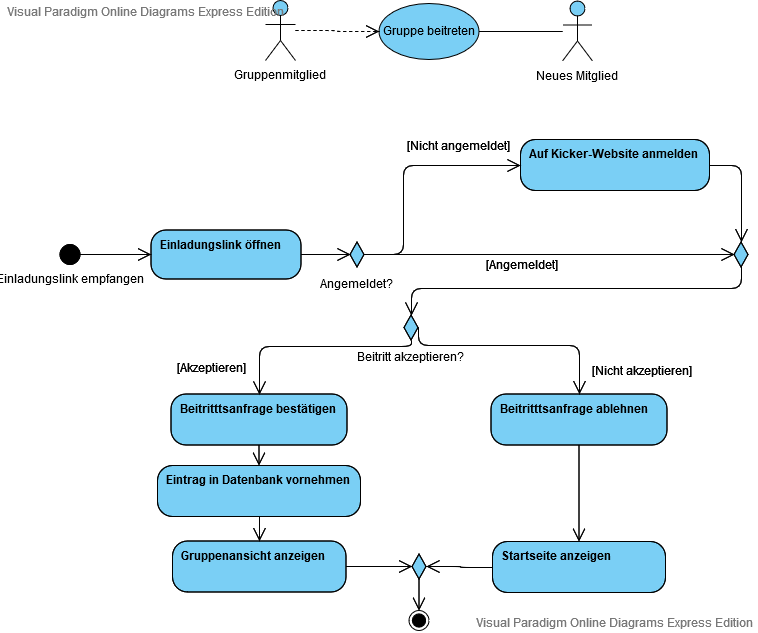
\includegraphics[width=\linewidth]{text/uc_ak_gruppenbeitritt.png}
	\caption{Use Case und Aktivitätsdiagramm: Gruppenbeitritt}
	\label{uc_ac_gruppenbeitritt}
\end{figure}
\begin{itemize}
	\item \textbf{Use Case:} Gruppe beitreten
	\item \textbf{Ziel:} Erfolgreicher Gruppenbeitritt
	\item \textbf{Kategorie:} Primär
	\item \textbf{Vorbedingung:} Nutzer hat ein Konto
	\item \textbf{Nachbedingung Erfolg:} Beitrittsanfrage annehmen
	\item \textbf{Nachbedingung Fehlschlag:} Beitrittsanfrage ablehnen
	\item \textbf{Akteure:} Gruppenmitglied, neues Mitglied
	\item \textbf{Auslösendes Ereignis:} Nutzer erhält Einladungslink
	\item \textbf{Beschreibung:} \begin{enumerate}
		\item Einladungslink öffnen
		\item Beitrittsanfrage bestätigen
		\item Eintrag in Datenbank vornehmen
		\item Gruppenansicht anzeigen
		\item Startseite anzeigen
	\end{enumerate}
	\item \textbf{Erweiterungen:} 1a. Auf Kicker-Website anmelden\\
	2b. Beitrittsanfrage ablehnen
	\item \textbf{Alternativen:} /
\end{itemize}



